\documentclass[../main.tex]{subfiles}

\begin{document}
\subsection{An overview of Intel SGX} % reference this to the developer reference
This section will not cover all of the details of SGX but only those applicable to our project, for a complete treatment
of SGX please refer to~\cite{IntelCorporation2010}. Intel SGX is a set of x86 instructions that allow for a programming model wherein a
program can be split into two components: an untrusted component that executes as normal and a trusted component that executes
within a protected area of RAM, called an enclave, which can only be accessed when executing the trusted component. 

The protection of an enclave is managed by the CPU; any data written to the enclave is encrypted first by a memory encryption engine (implemented in hardware) 
and is only decrypted when required by the CPU during the execution of the trusted component for which that enclave belongs. The key used for this encryption process
is derived from a combination of a device key, unique to each SGX-enabled CPU and the ``identity'' of the enclave called MRENCLAVE, a cryptographic hash of the enclave's contents
at the trusted component's initialization. SGX thus ensures that no process other than the one that initialized the enclave can access the protected area. 

Interacting with the trusted component, as a result, may only occur through invoking a programmer defined interface, called a callgate, as depicted in Figure~\ref{fig:sgxhighlevel}.

\begin{figure}[H]
	\centering
	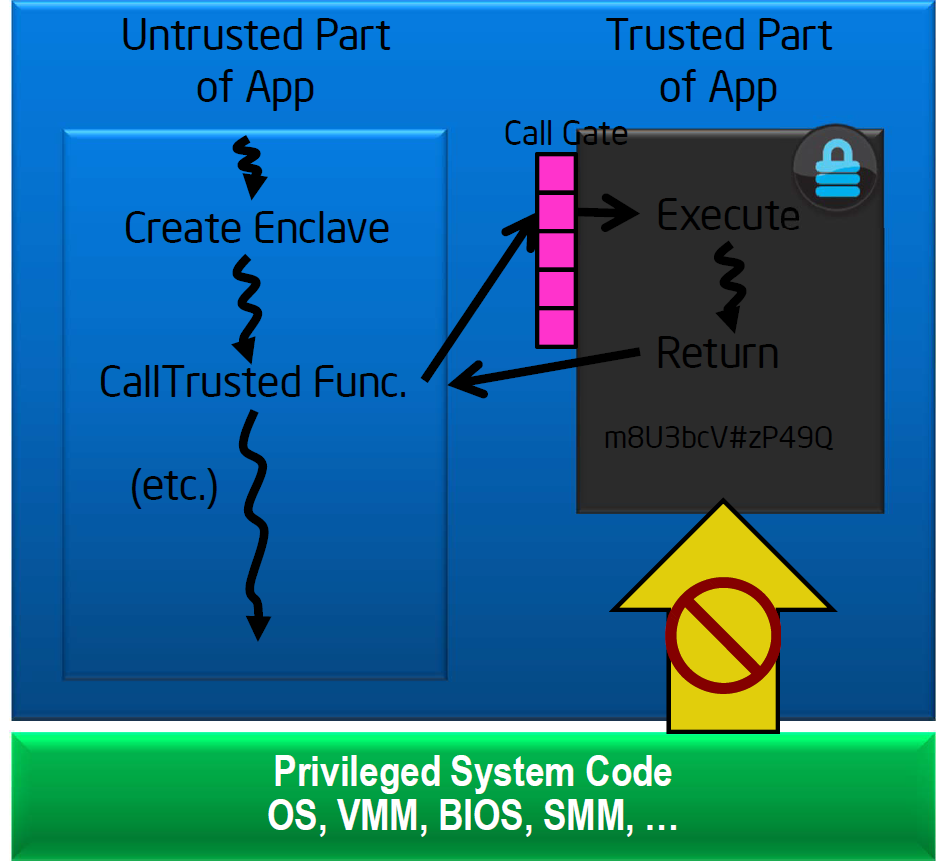
\includegraphics[scale=0.25]{images/sgxhighlevel.png}
	\caption{Interaction of the untrusted part of the application with the trusted part can only occur through a callgate}
	\label{fig:sgxhighlevel}
\end{figure}



\end{document}
